\documentclass{standalone}

\usepackage{gnuplot-lua-tikz}
\usepackage{tikz}
\usepackage{amssymb}
\usepackage{amsfonts}
\usepackage{mathrsfs}
\usepackage{amsmath}
\usepackage[amssymb]{SIunits}

\begin{document}
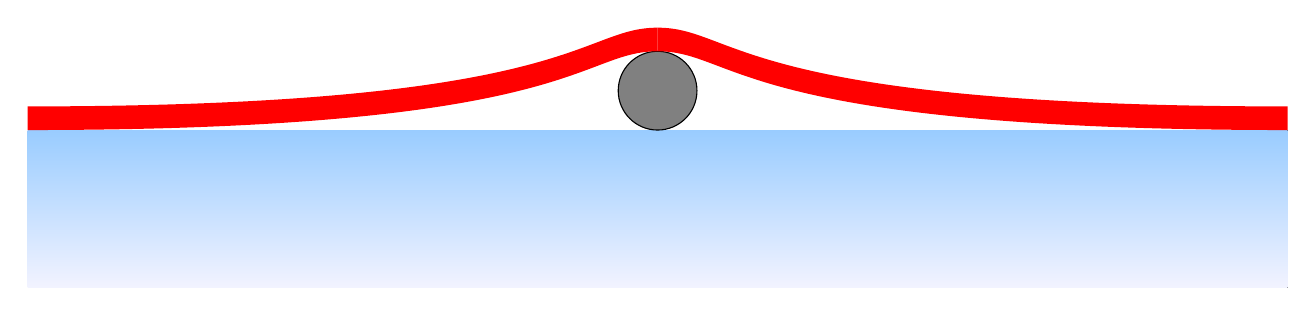
\begin{tikzpicture}[scale=1]

    % substrate
    \fill [shading=axis, bottom color=cyan!5!blue!5, top color=cyan!50!blue!40] (-8,0) rectangle (8,-2);


    \draw [fill=black!50] (0,0.5) circle (0.5);

    \fill [red] (0,1+0.3) .. controls +(-1,0) and +(7,0) .. (-8,0+0.3)  --  (-8,0) .. controls +(7,0) and +(-1,0.0) .. (0,1) -- cycle ;
    \begin{scope}[xscale=-1]
        \fill [red] (0,1+0.3) .. controls +(-1,0) and +(7,0) .. (-8,0+0.3)  --  (-8,0) .. controls +(7,0) and +(-1,0.0) .. (0,1) -- cycle ;
    \end{scope}

\end{tikzpicture}
\end{document}